
In this section, we describe the datasets, the environment we performed our experiments in, and the experiment designs along with their results.

\subsection{Environment}

In our experiments, we used a machine with 2.5 GHz Intel Xeon i7 processor, 128GB RAM, Java 1.8 SE Runtime Environment and R v3.3.2 on Ubuntu 16.04 operating system.

\subsection{Datasets}

We used three real world datasets to evaluate the performance and accuracy of our design.

\subsubsection{Dataset 1 - PocketData Dataset}
\label{sec:pocketdatadataset}

As the mobile workload dataset, we use an extended version of the PocketData~\cite{kennedy2015pocket} dataset which provides handset-based data directly collected from smartphones for multiple users.
It includes
%one month's
20 day's
trace of SQLite activity of
%11
\note{60}
PhoneLab~\cite{phonelab} smartphones running the Android smartphone platform. University at Buffalo's PhoneLab is a smartphone platform testbed consisting of 175 participants drawn from the university faculty, students and staff. They were provided a discounted Sprint service and a Google Nexus 5 smartphone to use as their primary device. In exchange, they ran a modified Android platform image containing custom instrumentation.

A 2013-14 survey indicates that PhoneLab participants are well distributed among genders and age brackets. ~\cite{phonelab} Because PhoneLab is open to any UB affiliate , the participants are in many different departments on campus, providing a reasonable level of on-campus spatial coverage. 

This dataset consists of various information about the usage patterns across a wide variety of apps, and is a best-effort anonymized dataset.
Most of the private information is irreversibly concealed but there are still some constants in the queries.

The older version of the dataset that includes a month's trace of SQLite activity of 11 users is available online~\cite{kennedy2015pocket}.
However, the data that we used in this paper is only available by request, and the researchers has to follow the IRB requirements of their institute to be able to use, and publish using this data.

\begin{table}[]
\centering
\caption{Dataset}
\label{tab:dataset}
\begin{tabular}{cc}
\textbf{Application}                                           & \textbf{\# of queries} \\ \hline
\begin{tabular}[c]{@{}c@{}}Complete\\ Dataset\end{tabular}     & 45,090,798 (tentative)             \\ 
Facebook                                                       & 1,272,779 (tentative)             \\
Google+                                                        & 2,040,793 (tentative)             \\
Hangouts                                                       & 974,349 (tentative)               \\
\begin{tabular}[c]{@{}c@{}}Google Play\\ Services\end{tabular} & 14,813,949 (tentative)            \\
Media Storage                                                  & 13,592,982 (tentative) \\ \hline          
\end{tabular}
\end{table}

\subsubsection{Dataset 2 - Controlled Dataset}
\label{sec:controlleddataset}

We collected this dataset in a controlled environment where one user's activities for one hour are recorded along with the time of each activity, and the activity the user performed. To create this dataset, we selected \emph{Facebook} application simply because it actively utilizes the mobile database, and we could define the descriptive activities such as opening a profile page, scrolling down on the home feed, and so on.

During the data collection period, the user was free to use the any other application along with Facebook, or not to use the phone at all. However, the user was informed about the experiment was being performed on Facebook application, and they should narrate what they are doing while doing it to be recorded. 

This dataset contains 60 minutes of queries that Facebook application issued to the database. There are \todo{about 5000} parsable~\footnote{by JSqlParser} queries recorded, labeled with what activity they were associated with, timing information of each query, and lastly the user labeled session which is roughly described to the user as \textit{``Session in an application is the period between a user starts to dedicate their attention to the application, and loses their interest.''} Note that this description is ambiguous, and aims to lead the experiment participant to form their understanding of a session.

\subsubsection{Dataset 3 - Controlled Activity}
\label{sec:controlledactivity}

This dataset contains queries that are generated when the user interacts with the mobile application for a specific purpose. While collecting these activity logs, everytime the user completes an operation, the set of queries issued is labeled with that certain activity.

For instance, on Facebook application, the user clicks on another profile on the feed page. This activity makes the application fire a sequence of queries. We capture these queries, and label them with the actual activity.

%Each line in the log has:

%\begin{itemize}
%  \item Device ID: Unique identifier for each device
%  \item UNIX timestamp: Milliseconds since 1970
%  \item Ordering: Timestamp and request order
%  \item Date and time: Human readable timestamp
%  \item Process ID: Standard UNIX process ID
%  \item Thread ID: Standard UNIX thread ID
%  \item Log level: Verbose (V), Debug (D), Info (I), Warning (W), Error (E) 
%  \item Tag: Source of log information, ``SQLite-Query-PhoneLab''
%  \item JSON object that holds various information about the event that is logged
%\end{itemize}

%information.

%Note that the app ID is not included in the log, because different apps can have the same process and thread IDs in different times.
%Our strategy to get the log lines for our app of interest is to search for the app name in JSON object parsing from the beginning of the file.
%When we first encounter the app of interest, we use process and thread IDs to identify the events related to that app until we encounter a different app name in the JSON object.

%Hence, we implement all the functions of the system with Java for it to be repackaged, and be able to be imported into mobile phones as well as servers.
%This may solve the privacy concerns of the users: allowing the processing to be performed on the phone instead of a company server even if it is not the ideal case due to performance and energy consumption constraints.

\subsection{Experiment Design}

The core expected output of the system presented in this paper is an expected query workload created based on the user's past activity without any supervision.
However, it is very difficult to answer the question of \textit{``what is the accuracy of such an output?''} without providing a comparison.
Therefore, we compare our session identification methodology with the state of the art of web query session identification, and also measure the accuracy of our session similarity method, we designed a supervised approach given in Section~\ref{sec:supervised} to be able to show the unsupervised approach presented has comparable results.

To achieve this, we designed the following experiments as building blocks to verify the accuracy and consistency of the methods that we use in each step.

\subsubsection{Experiment 1 - Clustering Accuracy}

In this experiment, we aim to measure the placement performance of clustering methodology described in Section~\ref{sec:profiler} over all of the queries in the query log.

We prepare ground truth cluster labels by manually inspecting all the unique queries within the query log for Facebook app. The accuracy of the clustering result is measured by comparing the query placements to the clusters to the ground truth.

\begin{table}[h!]
	\centering
	\caption{Clustering accuracy}
	\label{tab:clusteringAccuracy}
    \begin{tabular}{ccc}
    ~                                  & \textbf{Facebook} & \textbf{Google+} \\ \hline
    \# of queries                      & \#       & \#      \\
    \# of unique queries               & \#       & \#      \\
    \# of detected clusters            & \#       & \#      \\
    \begin{tabular}[c]{@{}c@{}}\# of accurately\\placed queries\end{tabular}    & \#       & \#      \\
    \begin{tabular}[c]{@{}c@{}}\# of inaccurately\\placed queries\end{tabular}  & \#       & \#      \\
    Accuracy                           & \#       & \#      \\ \hline
    \end{tabular}
\end{table}

For our experiments, we selected Facebook to be our example app. For visual purposes, we clustered the activities of only one user in Figure~\ref{fig:dendrogram}.
For this specific user's case, there are 84273 rows of activities in the log.
There are 8795 parsable select queries, however, there are only 59 unique queries among them.
Keep in mind that PocketData dataset is an anonymized dataset where most of the constant values are replaced with ``?'', which reduces the number of distinct queries greatly.
The dendrogram we created using Makiyama method and hierarchical clustering can be seen in Figure~\ref{fig:dendrogram}.

\begin{figure}[h!]
    \centering
    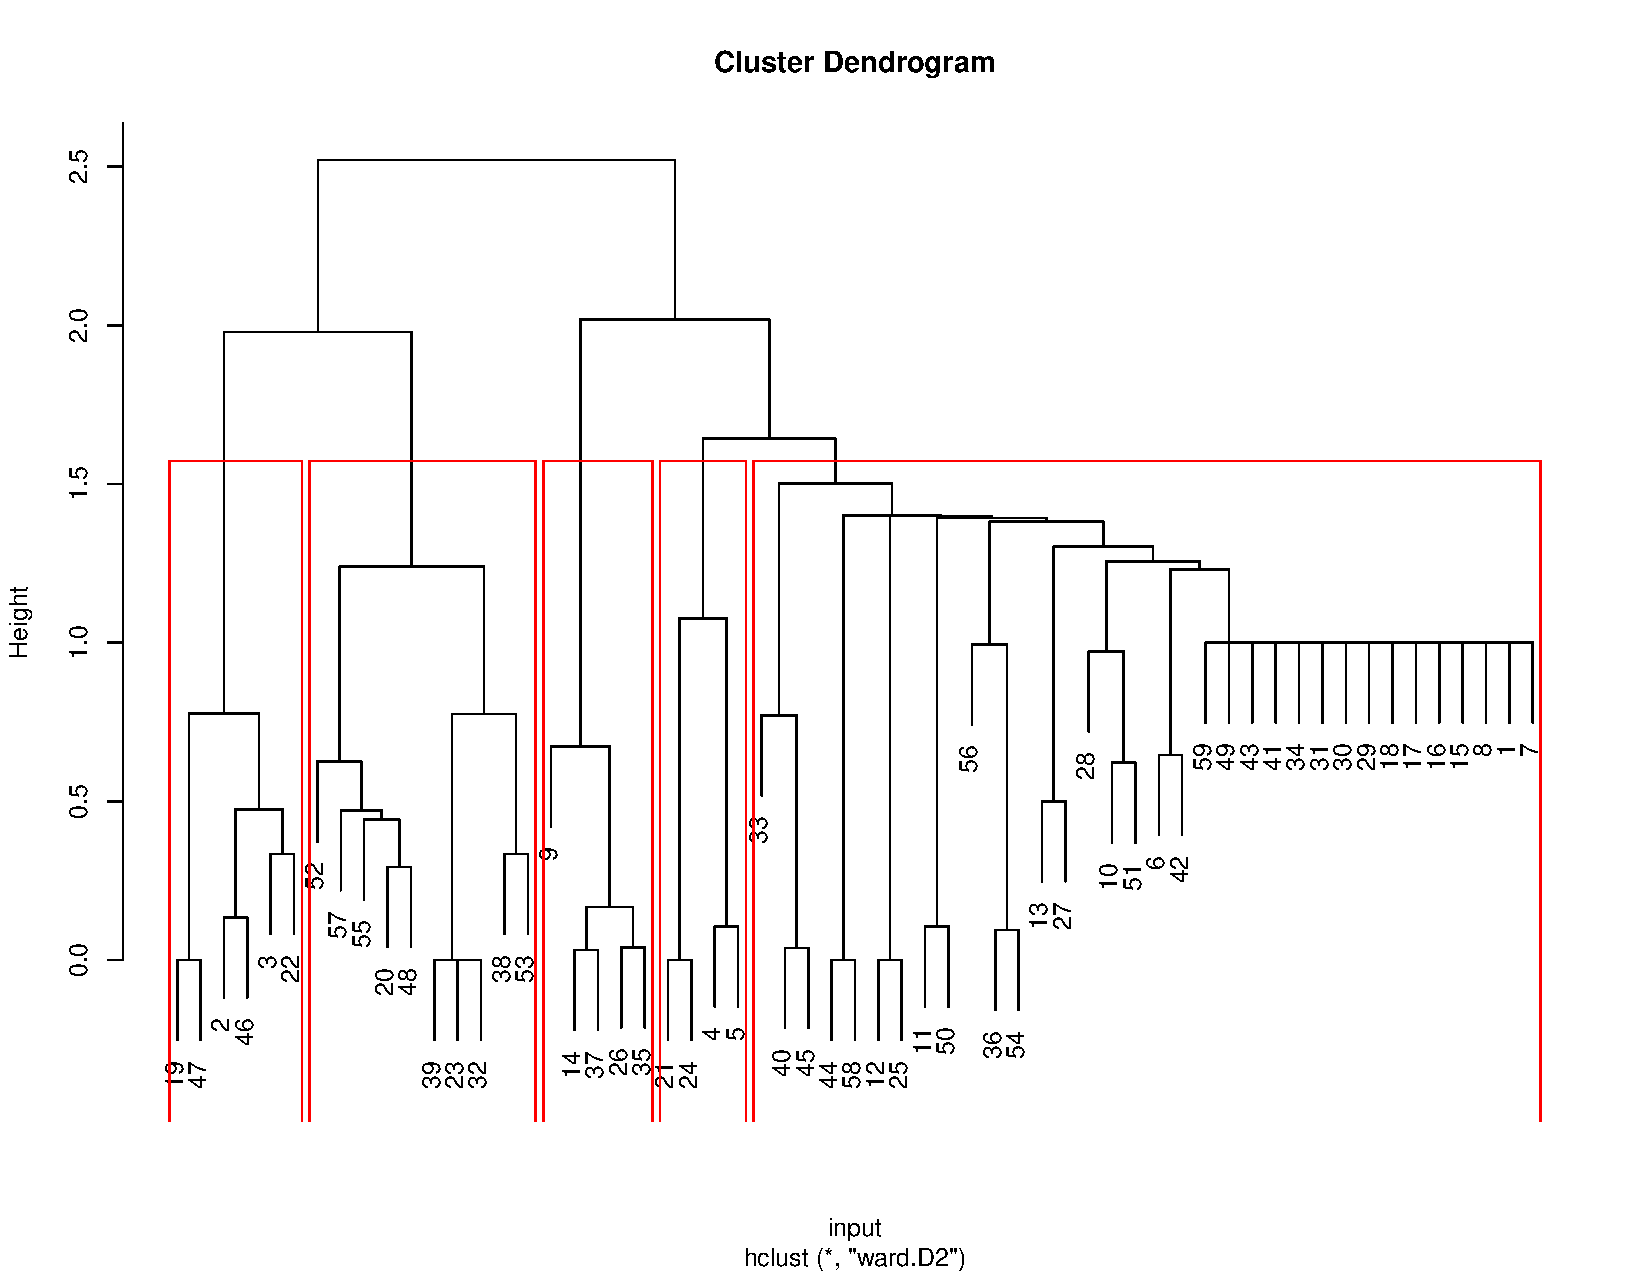
\includegraphics[width=0.5\textwidth]{graphics/User1}
    \caption{Clustering Dendrogram of Facebook usage for a user \todo{Renew}}
    \label{fig:dendrogram}
\end{figure}

As seen in Figure~\ref{fig:dendrogram}, there are 5 different clusters of queries when clustered with Makiyama method. In Table~\ref{tab:clusteringresult}, we provide the tasks performed by the queries within the corresponding cluster.

\begin{table}[h!]
\centering
\caption{Makiyama clustering results}
\label{tab:clusteringresult}
\begin{tabular}{cc}
\hline
\textbf{Cluster} & \textbf{Explanation}                        \\ \hline
1       & New notification check             \\ 
2       & Prefetch and retrieve notification \\ 
3       & Fill home feed                     \\ 
4       & Cache operations                   \\ 
5       & Housekeeping                       \\ \hline
\end{tabular}
\end{table}

%Also, for the n-gram approach, when we choose n to be 2, we created the clustering shown in Figure~\ref{fig:ngram}.

%\begin{figure}[h!]
%    \centering
%    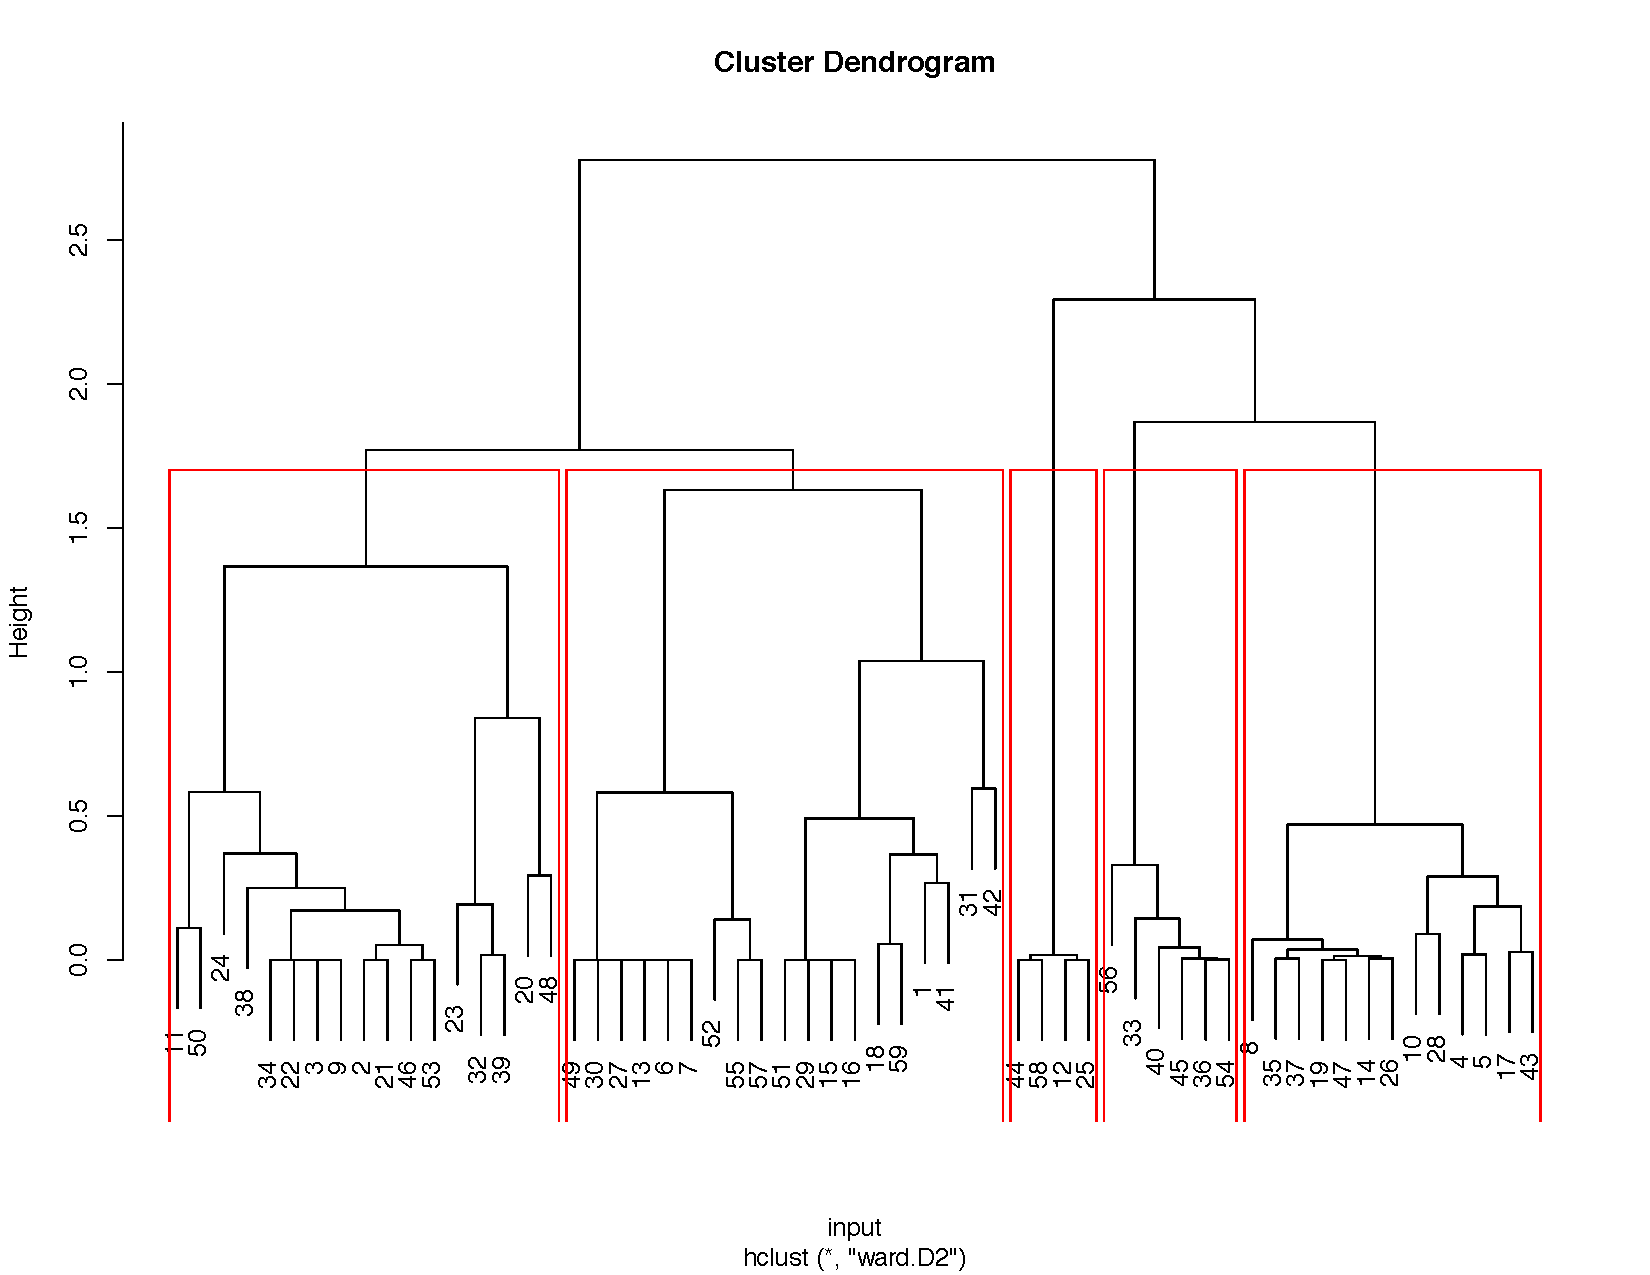
\includegraphics[width=0.5\textwidth]{graphics/Ngram}
%    \caption{N-Gram Clustering Dendrogram of Facebook usage for a user}
%    \label{fig:ngram}
%\end{figure}

%In Table~\ref{tab:clusteringresultngram}, we provide the explanations for the queries according to the clusters they got appointed with n-gram feature extraction scheme.

%\begin{table}[h!]
%\centering
%\caption{N-Gram clustering results}
%\label{tab:clusteringresultngram}
%\begin{tabular}{cc}
%\hline
%\textbf{Cluster} & \textbf{Explanation}                       \\ \hline
%1       & Key-Value lookups                 \\ 
%2       & No filter or multiple row lookups \\ 
%3       & Lookup in a provided list         \\ 
%4       & Complex queries                   \\ 
%5       & Top-k row queries                 \\ \hline
%\end{tabular}
%\end{table}

%We also created a tanglegram to show how similar clusterings these two methods created in Figure~\ref{fig:tanglegram}. As can be seen in the figure, there is little to no similarity between these clusterings which is not unexpected since the two feature extraction mechanisms completely have different strategies and targets different features.

We also created a tanglegram to show how the automated clusterings, and manual cluster assignments match in Figure~\ref{fig:tanglegram}.
%As can be seen in the figure, there is little to no similarity between these clusterings which is not unexpected since the two feature extraction mechanisms completely have different strategies and targets different features.

\begin{figure}[h!]
    \centering
    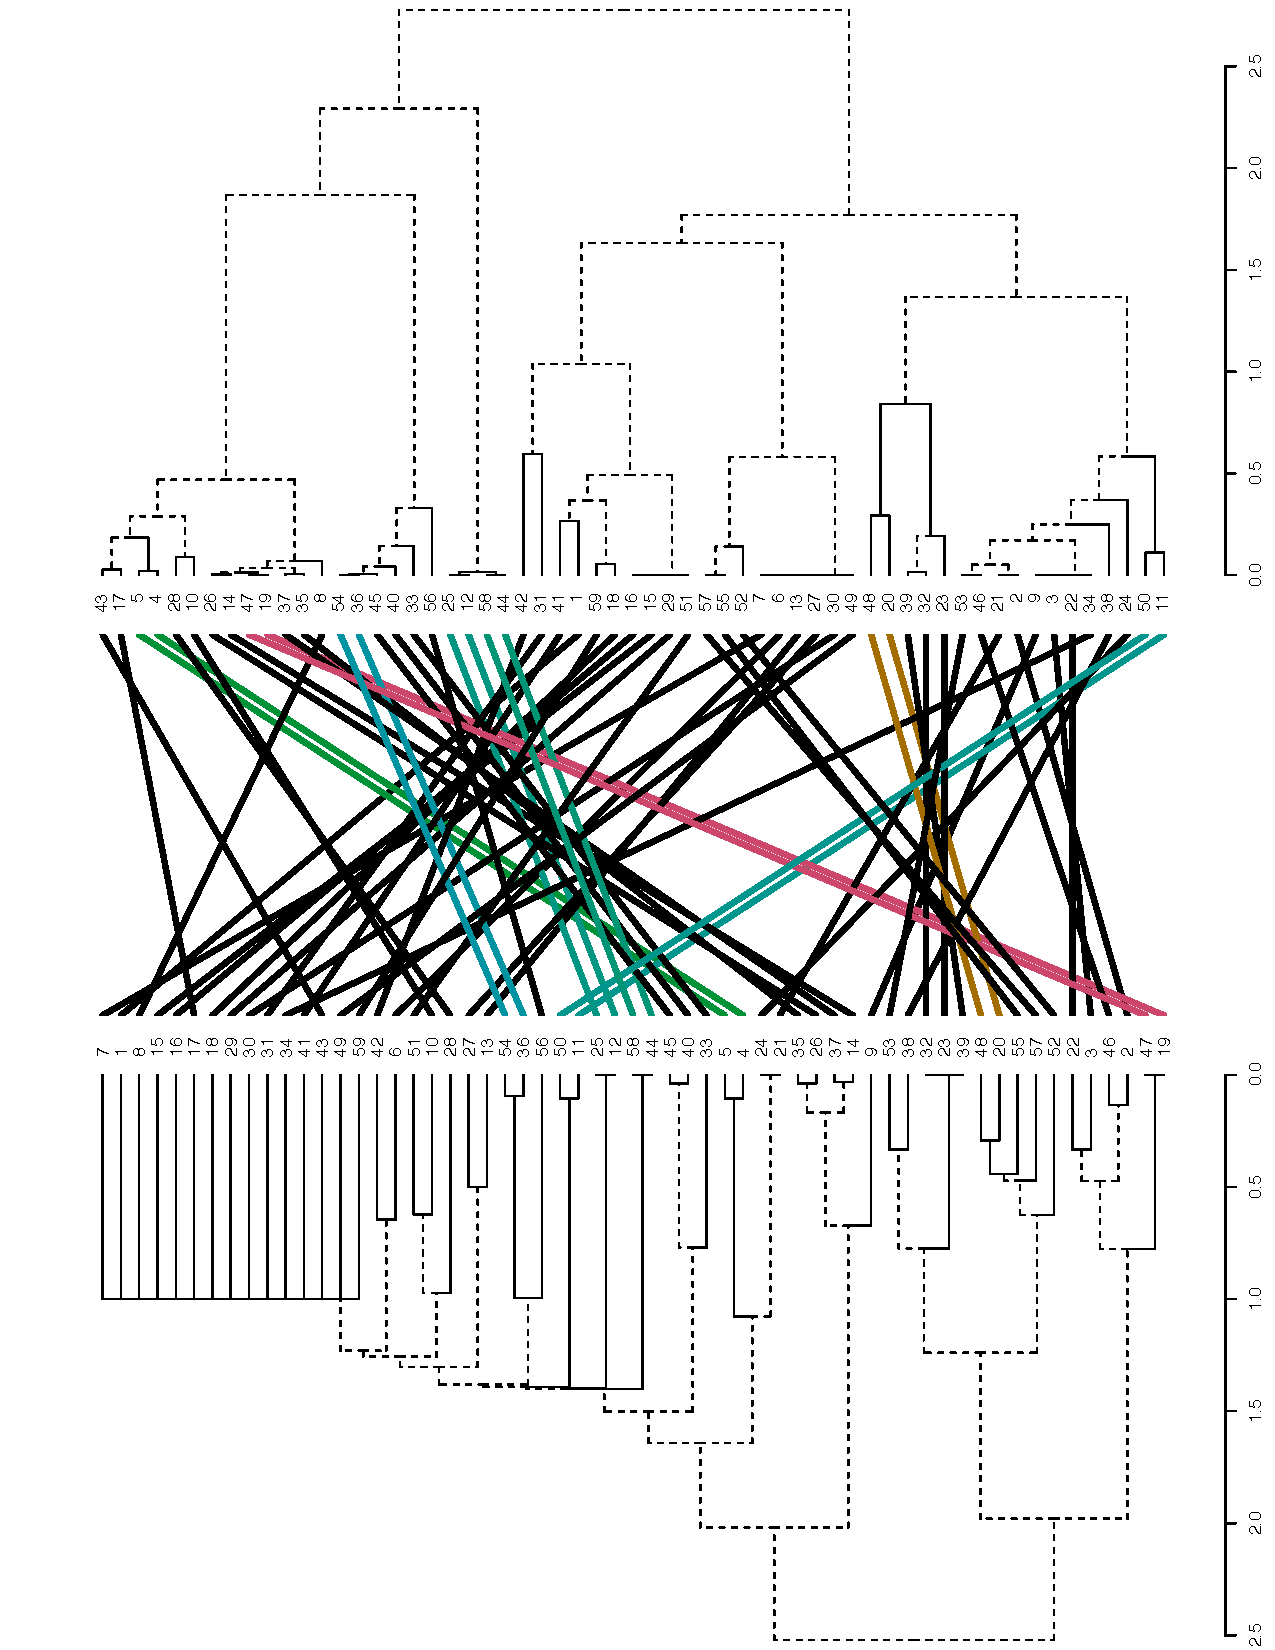
\includegraphics[width=0.45\textwidth]{graphics/tanglegram}
    \caption{Matching of manual clustering and Makiyama clustering \todo{Renew}}
    \label{fig:tanglegram}
\end{figure}

\subsubsection{Experiment 2 - Idle Time Tolerance}
This set of experiments were directed towards coming up with an idle time tolerance for each user.
We ran our user session segmentation routine described in Section~\ref{sec:sessionidentifier} for query logs of all users for all the query workload they created.

The idle time tolerances used were 10ms, 100ms, 1s, 5s, 10s, 1min, 2min and 5min.
So, we chose an idle time specific to each user for our further experiments.

% \begin{figure}[h!]
%     \centering
%     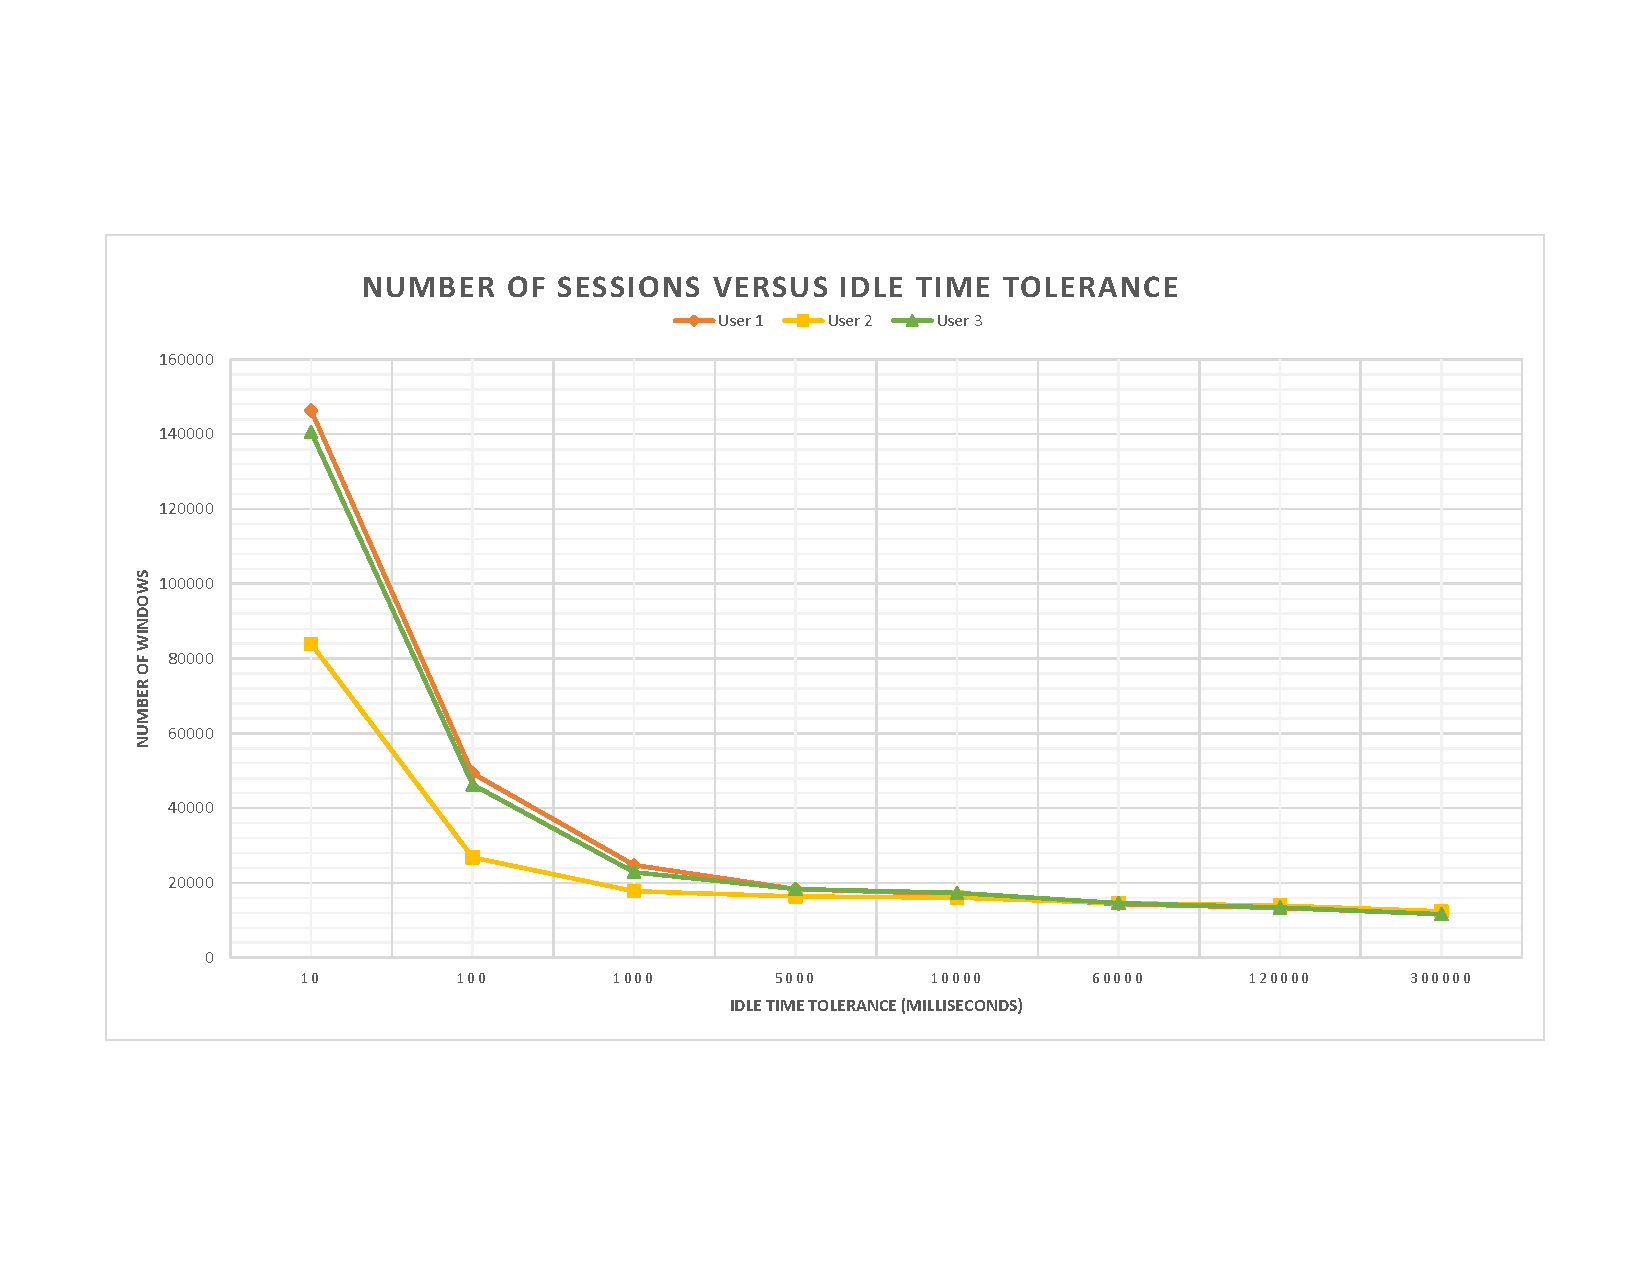
\includegraphics[width=0.45\textwidth]{graphics/IdleTimeTolerances}
%     \caption{\todo{Renew: Create new table for all users with the new data. Show cutoff points clearly.} Number of user sessions generated with varying idle time tolerances}
%     \label{fig:idletime}
% \end{figure}
\todo{Create new table for all users with the new data. Show cutoff points clearly.}

\subsubsection{Experiment 3 - Session Identification on Controlled Dataset}

The controlled dataset is created by monitoring and labeling every activity performed on the phone. Hence, both applying the state of the art search log session identification technique described in Section~\ref{sec:backgroundSessionIdentification} and our heuristic. \note{Of course, this experiment here cannot be used to conclude our method is better than the cascade method. It is just an indicator that it is more suitable for mobile workloads.}

The controlled dataset includes \todo{13} labeled sessions. Our methodology identified \todo{12} sessions, where one of the sessions was labeled to be the tail end of the previous session. Hagen \textit{et al.}~\cite{hagen2011query} methodology, on the other hand, identified only \todo{3} sessions, where \todo{2} of these sessions were correctly identified, but the \todo{one} of the sessions identified covered \todo{11} user labeled sessions. This result confirms that although the state of the art method for web search query session identification method is successful in the area it is developed for, it is not suitable for mobile phone database session identification. 

\subsubsection{Experiment 4 - Activity Recognition Performance}
The aim of this experiment is to measure the accuracy of various activity detection techniques using labeled data. We collected one hour of Facebook query log where the user recorded every activity they performed freely on the phone with corresponding time data as described in Section~\ref{sec:controlleddataset}. We then collected the query output of a set of activities individually.

\begin{figure}[h!]
    \centering
    \includegraphics[width=0.45\textwidth]{graphics/activityRecognition}
    \caption{Activity recognition performance for different profiler methods \todo{Renew}}
    \label{fig:activityRecognition}
\end{figure}

Figure~\ref{fig:activityRecognition} shows that feature based KL-Divergence method and query clustering methods have comparable accuracy results. 

\todo{We can test different tresholds and add a ROC graph for each method. It would make this claim stronger, and eliminate any questions that the reviewers can raise.}


\subsubsection{Experiment 5 - Supervised vs Unsupervised Common Pattern Recognition on PocketData Workload}

\todo{Warning! This subsection will be filled with new results!}

Extracting meaningful patterns from user data is central to a reliable characterization of the smartphone database workload. We proposed a robust session similarity measure which takes into the account the considerations and constraints that are imposed by the problem domain. We believe that our experimental results support the dependability of this approach for mobile applications. 

We applied the idle time treshold specific for each user over the Facebook query workload as we indicated in the previous section in order to determine how many sessions there are. \todo{Rewrite this: This operation revealed that there were 15820 sessions initiated in the dataset according to the session definition. Among these 15820 sessions, 5184 of them had 90\% or higher average similarity with all other sessions and there are 25 sessions that had 25\% or less average similarity with all other sessions as show in Figure~\ref{fig:averagesimilarity}.}

We believe that a random session selection among the 5184 sessions can provide us with a representative query set of the workloads for all users since 90\% average similarity means the query set represents 90\% of all the sessions in the dataset. The average, minimum and maximum session lengths are given in Table~\ref{tab:sessionlength}.

\begin{figure}[h!]
    \centering
    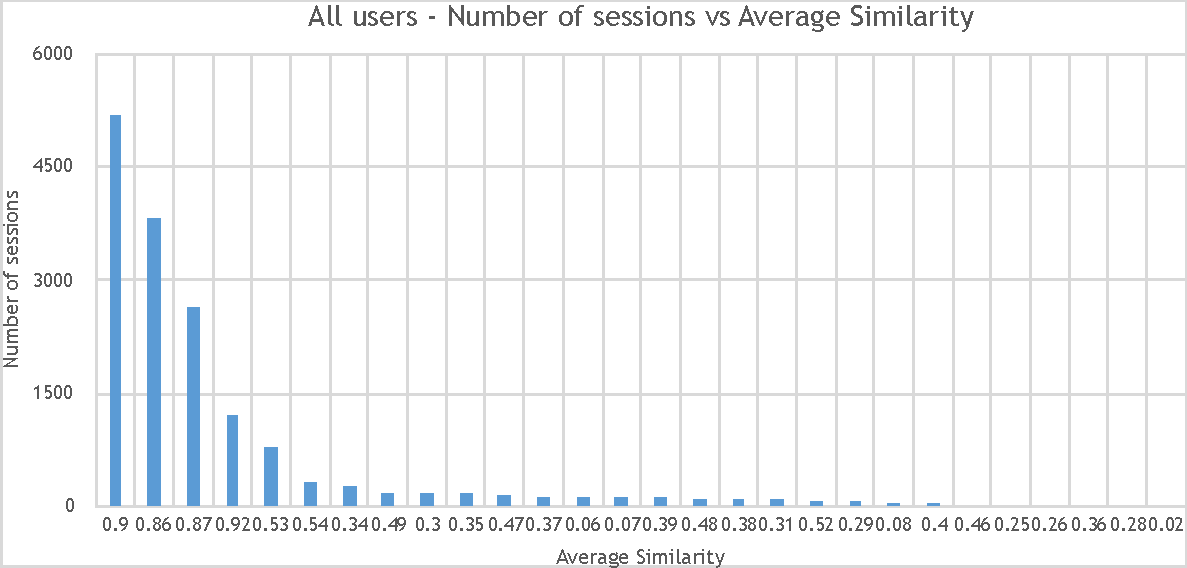
\includegraphics[width=0.45\textwidth]{graphics/allsessions}
    \caption{Number of sessions separated by their average similarity \todo{Will be replaced with supervised and unsupervised method performance comparison graph}}
    \label{fig:averagesimilarity}
\end{figure}

\begin{table*}[h!]
\centering
\caption{Session length}
\label{tab:sessionlength}
\begin{tabular}{ccccl}
\cline{1-4}
\multicolumn{1}{|c|}{}                                        & \multicolumn{1}{c|}{Average Session Length} & \multicolumn{1}{c|}{Minimum Session Length} & \multicolumn{1}{c|}{Maximum Session Length} &  \\ \cline{1-4}
\multicolumn{1}{|c|}{Sessions with 90\% or higher similarity} & \multicolumn{1}{c|}{3474.32 ms}                      & \multicolumn{1}{c|}{10 ms}                      & \multicolumn{1}{c|}{159320 ms}                      &  \\ \cline{1-4}
\multicolumn{1}{|c|}{Sessions with 25\% or less similarity} & \multicolumn{1}{c|}{2402.91 ms}                      & \multicolumn{1}{c|}{4 ms}                      & \multicolumn{1}{c|}{136110 ms}                      &  \\ \cline{1-4}
\multicolumn{1}{|c|}{All sessions}                            & \multicolumn{1}{c|}{5065.02 ms}                      & \multicolumn{1}{c|}{4 ms}                      & \multicolumn{1}{c|}{218959 ms}                      &  \\ \cline{1-4}
\multicolumn{1}{l}{}                                          & \multicolumn{1}{l}{}                        & \multicolumn{1}{l}{}                        & \multicolumn{1}{l}{}                        & 
\end{tabular}
\end{table*}

As for outlier detection, the 25 sessions that have 25\% or less average similarity is a very moderate number that should be inspected to understand the structure of extraordinarily different sessions.

\todo{Go on here, add results...}





